\documentclass[fleqn,10pt]{article}
%\usepackage[a4paper, margin=1.1in]{geometry}
\usepackage{amssymb,amsmath}
\usepackage{mathpartir}
\usepackage{doc/saoithin}
\usepackage{tikz}
\usepackage{tikz-cd}
\usetikzlibrary{arrows,matrix}
\usepackage{graphicx}
\usepackage{epstopdf}

\def\includepicture#1{\includegraphics{#1.eps}}

\parindent=0pt % I hate first line indentation
\parskip=3pt   % I like a visual white gap between paragraphs


\author{%
  Andrew Butterfield%
  \and
  Arthur Hughes
}
\title{Theoretical Aspects of UTP}
\date\today

\def\TODO#1{%
  \textbf{ToDo: }
  \textit{#1}
}

\begin{document}

\bibliographystyle{alpha}

\maketitle
\tableofcontents

\section{Introduction}

This document is a collection of theoretical musings regarding the UTP.

\newpage
\section{Kleisli Relations}

\def\F{\mathsf{F}}
\def\E{\mathsf{E}}
\def\id{\mathrm{id}}
\def\H{\mathbf{H}}
\def\He{\mathbb{H}}

\subsection{The Kleisli Triple}

The general notion of a Kleisli triple $(\F,\eta,\_^*)$:
\begin{eqnarray*}
   \F      &:& Type \fun Type
\\ \eta_A &:& A \fun \F A
\\ \_^*   &:&  (A \fun \F B) \fun (\F A \fun \F B)
\end{eqnarray*}
which,
given $ f : A \fun \F A $ and $g : B \fun \F C $
for arbitrary types $A$, $B$ and $C$,
must satisfy the following laws:
\begin{eqnarray*}
   \eta_A^*      &=& \id_{\F A}
\\ f             &=& f^* \circ \eta_A
\\ g^* \circ f^* &=& (g^* \circ f)^*
\end{eqnarray*}
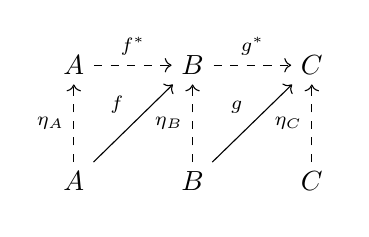
\begin{tikzpicture}
  \matrix [matrix of math nodes,column sep=1cm,row sep=1cm]
  {
    |(TA)| \F A  &  |(TB)| \F B  &  |(TC)| \F C  \\
    |(A)|   A   &  |(B)|   B   &  |(C)|   C   \\
  } ;
  \tikzstyle{every node}=[midway,auto,font=\scriptsize]
  \draw [->]        (A) -- node {$f$} (TB) ;
  \draw [->,dashed] (A) -- node {$\eta_A$} (TA) ;
  \draw [->]        (B) -- node {$g$} (TC) ;
  \draw [->,dashed] (B) -- node {$\eta_B$} (TB) ;
  \draw [->,dashed] (C) -- node {$\eta_C$} (TC) ;
  \draw [->,dashed] (TA) -- node {$f^*$} (TB) ;
  \draw [->,dashed] (TB) -- node {$g^*$} (TC) ;
\end{tikzpicture}

\subsection{Non-deterministic $\F$}

A common form of non-homogeneous theory in UTP is one that relates
some system state $S$ to some form of $S$ with ``effects'', written as $\E S$.
\[
  S \rel \E S
\]
This is typically isomorphic, given a healthiness condition $\H$ to:
\[
  S \fun \H(\power(\E S))
\]
Here we take healthy sets of effects,
denoting a (demonic) non-deterministic choice among those effects.

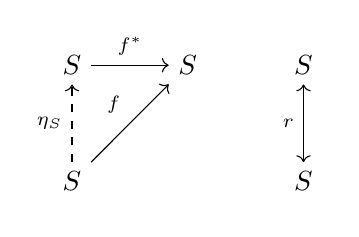
\begin{tikzpicture}
  \matrix [matrix of math nodes,column sep=1cm,row sep=1cm]
  {
    |(PFS0)| \power\E S  &  |(PFS1)| \power\E S  &  |(FS)| \E S  \\
    |(S)|   S            &                       &  |(S2)|   S   \\
  } ;
  \tikzstyle{every node}=[midway,auto,font=\scriptsize]
  \draw [->,dashed] (S) -- node {$\eta_S$} (PFS0) ;
  \draw [->]        (S) -- node {$f$} (PFS1) ;
  \draw [->]        (PFS0) -- node {$f^*$} (PFS1) ;
  \draw [<->]        (S2) -- node {$r$} (FS) ;
\end{tikzpicture}

Here we expect the following to hold true:
\[
  (s,e) \in r \quad\equiv\quad e \in f(s)
\]

Examples for $\H(\power(\E S))$ include:
\begin{eqnarray*}
   \He(S \fun [0,1]) && \mbox{Probability, He et. al.}
\\ \power(\power S)) && \mbox{Angelic Choice}
\end{eqnarray*}

We are interested in exploring the connection between
the non-homogeneous relation
\[ S \rel \E S\]
(or its functional form $S \fun \power(\E S)$)
and the homogeneous relation
\[ \E S \rel \E S \]
(also viewed functionally as $\E S \fun \power(\E S)$.

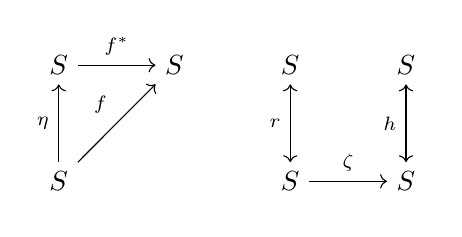
\begin{tikzpicture}
  \matrix [matrix of math nodes,column sep=1cm,row sep=1cm]
  {
    |(PFS0)| \power\E S  &  |(PFS1)| \power\E S  &  |(FS)| \E S & |(FS2)| \E S \\
    |(S)|   S            &                       &  |(S2)|   S  & |(FS3)| \E S  \\
  } ;
  \tikzstyle{every node}=[midway,auto,font=\scriptsize]
  \draw [->]  (S)    -- node {$\eta$} (PFS0)  ;
  \draw [->]  (S)    -- node {$f$}     (PFS1) ;
  \draw [->]  (PFS0) -- node {$f^*$}   (PFS1) ;
  \draw [<->] (S2)   -- node {$r$}     (FS)   ;
  \draw [<->] (FS3)  -- node {$h$}     (FS2)  ;
  \draw [->]  (S2)   -- node {$\zeta$} (FS3)  ;
\end{tikzpicture}

This is not a simple example of a Kleisli Triple,
given $f : S \fun \power (\E S)$,
as here we want a lifted function from
$\E S$, and not $\F S$.
Note that here we have $\eta = \setof\_ \circ \zeta$, where $\setof\_$ is the
singleton-set injection operator.

In particular, it is not clear how $h$ is derived from $f$.
Certainly we can link
\[
 e \in f(s)
 \qquad \mbox{and} \qquad
 (s,e) \in r
\]
with
\[
  (\zeta(s),e) \in h
\]
What is the link? What choices do we have?
How does it extend to the general case $(e_s,e) \in h$
where $e_s$ is not in the image of $\zeta$ ?

One possibility is to define $h$ as:
\[
  h  \defs  \zeta^\circ ; r
\]
where $\_^\circ$ is relational converse, and $;$ is relational composition.
The question now is, how to extend $\zeta^\circ$ to elements of $\E S$ not in
the relational image $\zeta(S)$. How does this extension depend on the nature of
$\E$?


\newpage
\bibliography{doc/SAOITHIN}

\end{document}
